% REMEMBER TO SET LANGUAGE!
\documentclass[a4paper,10pt,english]{article}
\usepackage[utf8]{inputenc}
\usepackage[english]{babel}
% Standard stuff
\usepackage{amsmath,graphicx,varioref,verbatim,amsfonts,geometry}
% colors in text
\usepackage[usenames,dvipsnames,svgnames,table]{xcolor}
% Hyper refs
\usepackage[colorlinks=false]{hyperref}

% Document formatting
\setlength{\parindent}{0mm}
\setlength{\parskip}{1.5mm}

%Color scheme for listings
\usepackage{textcomp}
\definecolor{listinggray}{gray}{0.9}
\definecolor{lbcolor}{rgb}{0.9,0.9,0.9}

%Listings configuration
\usepackage{listings}
%Hvis du bruker noe annet enn python, endre det her for å få riktig highlighting.

\lstdefinelanguage{python}
{
	morekeywords={print,abs,for,def,if,while,do,break,return,from,import,try,except,else,elif},
	sensitive=false,
	morecomment=[l]{\#}
}

\lstset{language=python,
	backgroundcolor=\color[rgb]{.95,.95,.95},
	numbers=left,xleftmargin=10pt,
	numberstyle=\tiny,stepnumber=1,numbersep=5pt,
	stringstyle=\color{red},
	basicstyle=\footnotesize \ttfamily,
	keywordstyle=\color{blue},
	commentstyle=\color{green},
	basewidth=0.60em,
	showstringspaces=false,
	captionpos=b,
	frame=single
}

\newcounter{subproject}
\renewcommand{\thesubproject}{\alph{subproject}}
\newenvironment{subproj}{
\begin{description}
\item[\refstepcounter{subproject}(\thesubproject)]
}{\end{description}}

%Lettering instead of numbering in different layers
% \renewcommand{\labelenumi}{\alph{enumi}}
\renewcommand{\thesubsection}{\roman{subsection}}
\renewcommand{\thesection}{\alph{section}}

%opening
\title{FYS-MEK1110 - Mandatory assignment 4}
\author{William Dugan}

\begin{document}

\maketitle

\section{}
We are going to sketch the function
\begin{equation}
U(x) = 
    \left\{\begin{matrix}
    U_0, & |x| \geq x_0 \\ 
    U_0 \frac{|x|}{x_0}, & |x| < x_0
    \end{matrix}\right.
\end{equation}

\begin{figure}[h!]
    \centering
    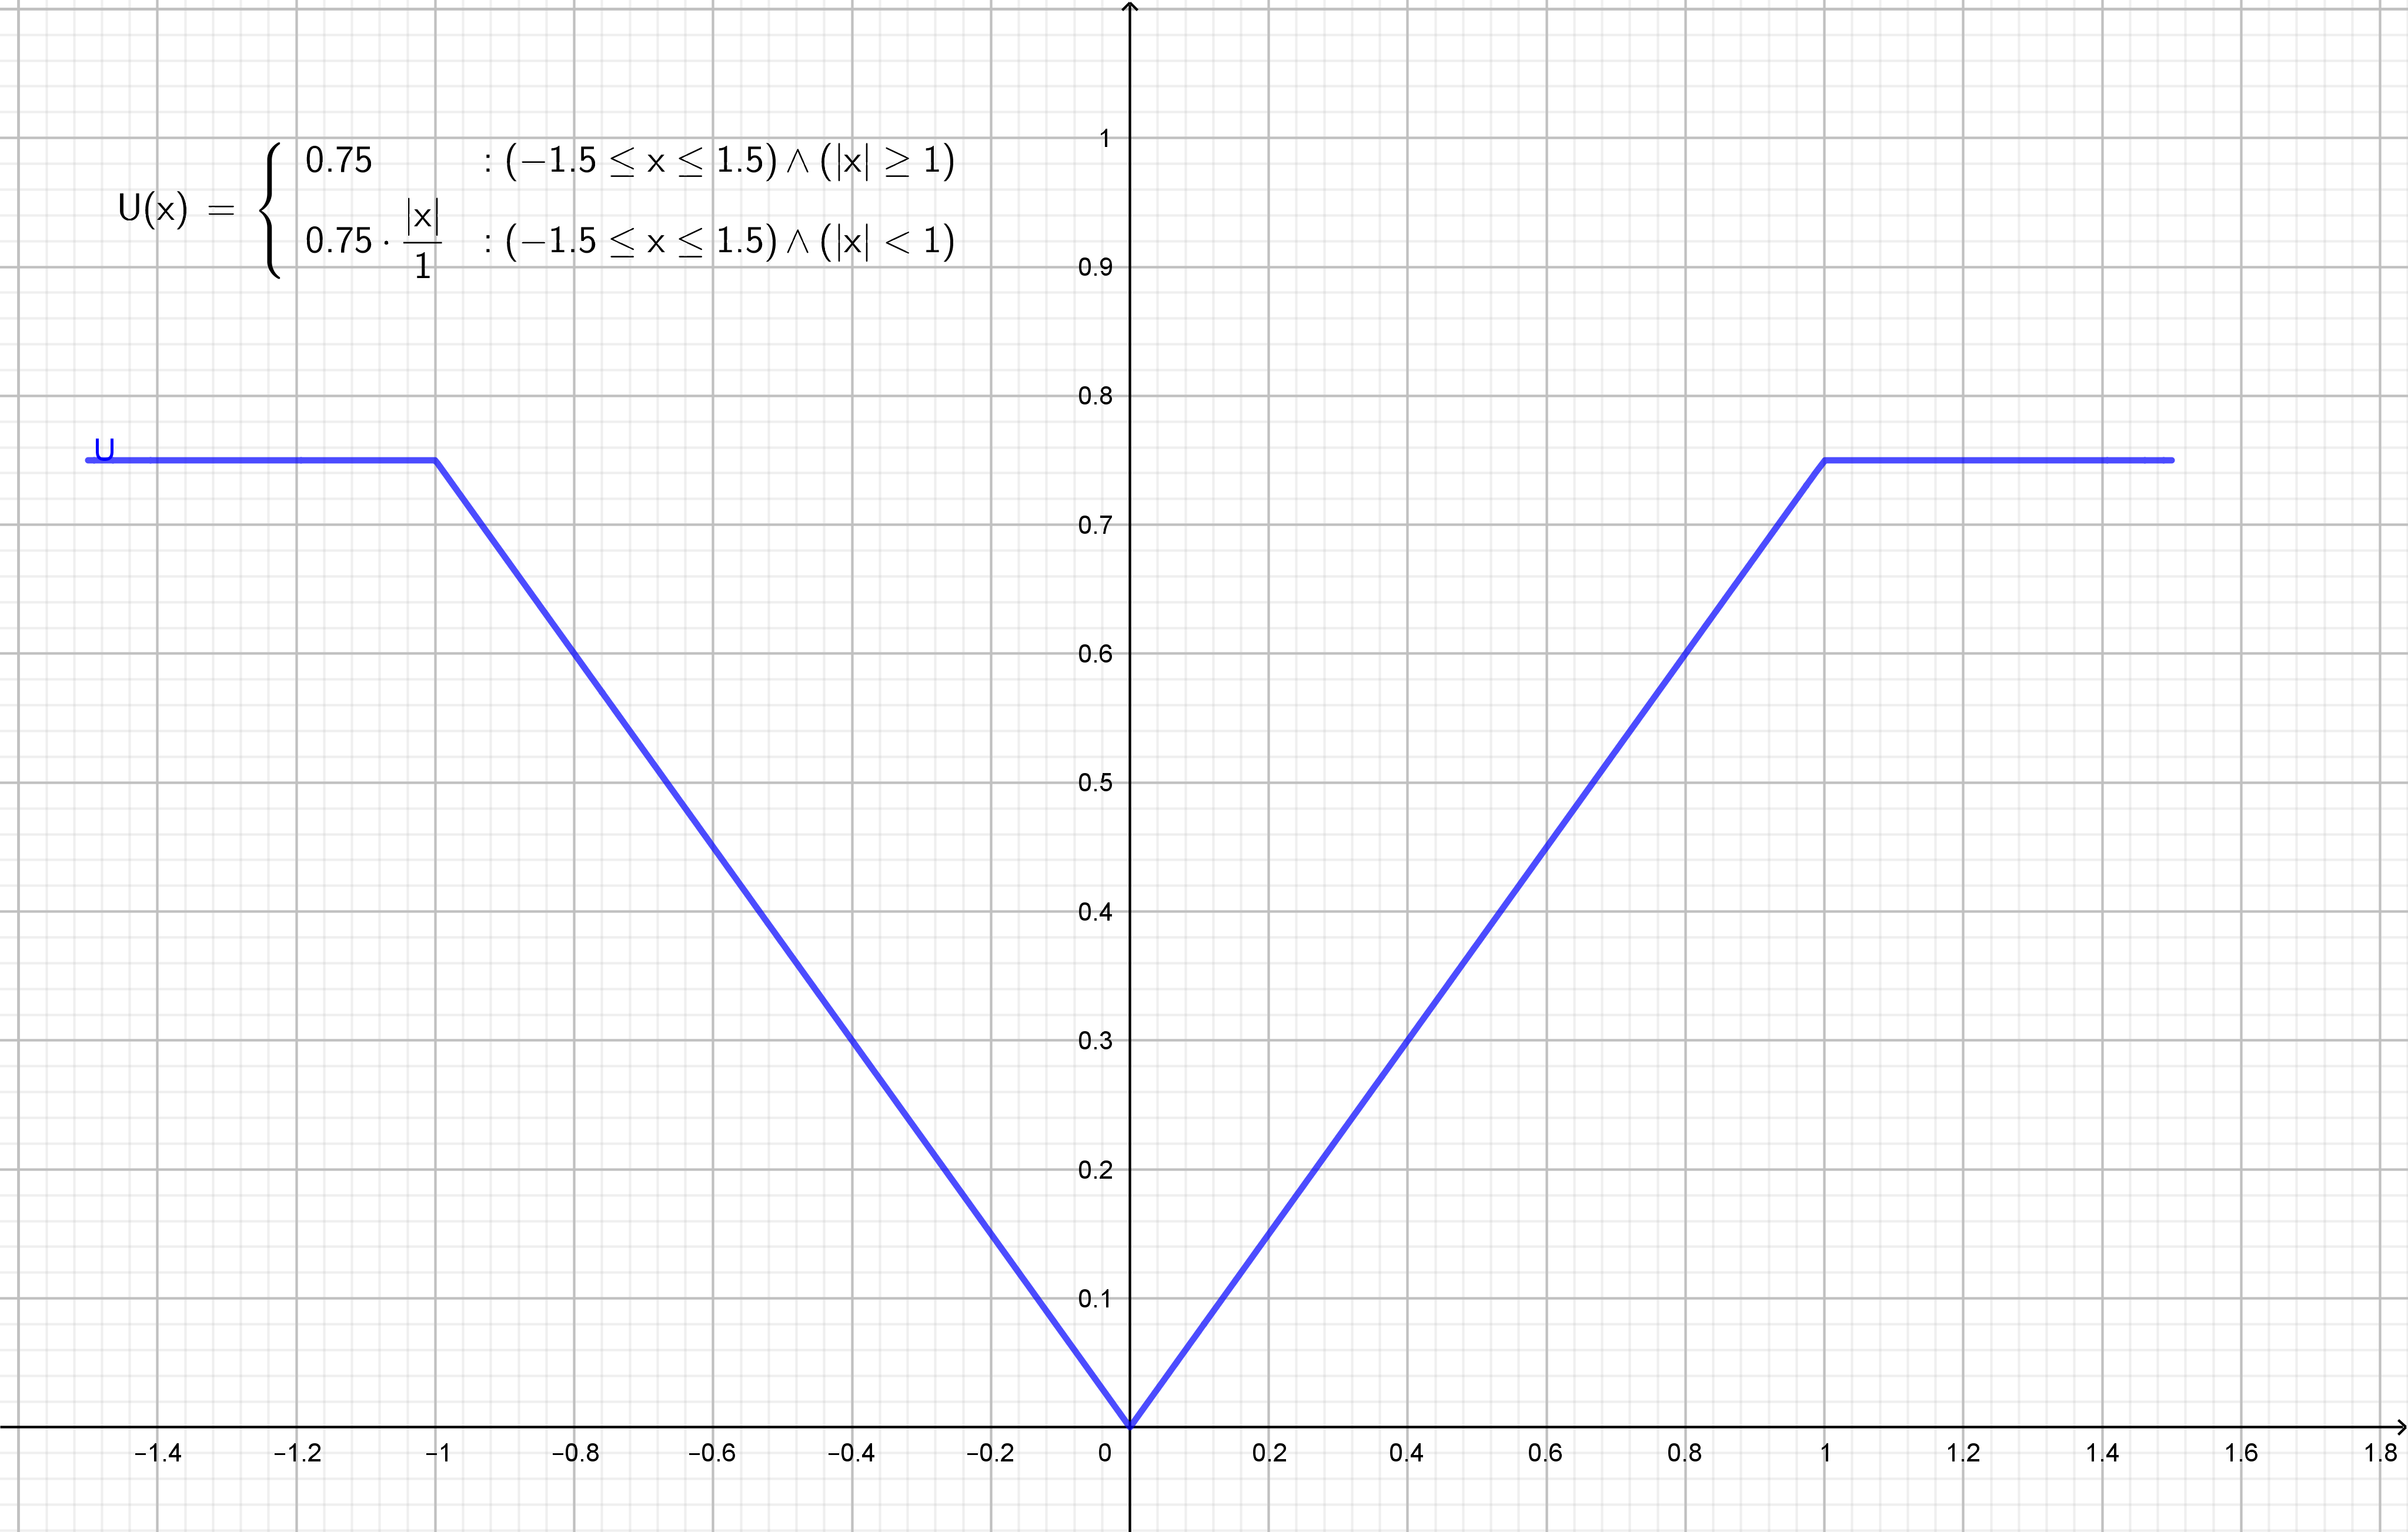
\includegraphics[scale=0.4]{figure_a.png}
    \caption{U(x) plotted for $x\in[-1.5, 1.5]$ with $U_0 = 0.75, x_0 = 1$.}
    \label{fig:fig_a}
\end{figure}

We have three equilibrium points, at $x=\pm x_0$ and $x=0$. The point in $x=0$ is a stable equilibrium point as the potential is at a minimum. The other are unstable as the potential is at maximum. We can use the relation $E_{atom, total} = KE_{atom} + PE_{atom}$. If $E_{atom, total} \geq PE_{atom}$ the atom will escape the trap, else it will stay inside the trap. 

\section{}
To find the force on the atom due to the field we use 
\begin{equation}
    F = - \nabla U
\end{equation}
In one dimension, we get $F = - \frac{dU}{dx}$. Hence
\begin{equation}
F(x) = 
    \left\{\begin{matrix}
    0, & x=0, |x| \geq x_0 \\ 
    -\frac{U_0}{x_0} \frac{x}{|x|}, & 0 < |x| < x_0
    \end{matrix}\right.
\end{equation}

Since the force on the atom due to the field can be written as a gradient of a potential, it is per definition a conservative force.

\section{}
Since $\sum F_{ext} = 0$ we can use conservation of energy to find the velocity of an atom with mass $m$ and $v_0 = \sqrt{4U_0/m}$ at $x=x_0/2$ and $x=2x_0$.

\begin{align*}
    E_1 &= E_0 \\
    \frac{1}{2}m v^2 + U(x) &= \frac{1}{2}m v_0^2 \\
    v^2 &= \frac{4U_0}{m} - \frac{2}{m}U(x) \\
    v &= 
    \pm \sqrt{
        \frac{2}{m}(2U_0 - U(x))
    }
\end{align*}
for $x=x_0/2$ we get $v=\sqrt{3U_0/m}$ and for $x=2x_0$ we get $v=\sqrt{2U_0/m}$.

\section{}
If we change the sign of our $x$-value, we simply change the sign of the velocity. Hence, for $x=-x_0/2$ we get $v=-\sqrt{3U_0/m}$ and for $x=-2x_0$ we get $v=-\sqrt{2U_0/m}$.

\section{}
If $KE=0$ at $x=0$ the electrostatic force $F_0$ must be greater or equal to $F(x_0)$ in order for the atom to escape. This gives $|F_0| > U_0/x_0$.

\newpage
\section{}
We introduce the force
\begin{equation}
    F = - \alpha v
\end{equation}
for $|x|< x_0$. The force depends on the velocity of the atom, which means that it depends on the path the atom takes. This makes it non-conservative.

\section{}
To find the acceleration:
\begin{align*}
    \sum F &= ma \\
    F_0 + F(x) &= ma \\
    a &= \frac{F_0 + F(x)}{m}
\end{align*}
If we insert our expressions we get
\begin{equation}
a(x) = 
    \left\{\begin{matrix}
    0, & x=0, |x| \geq x_0 \\ 
    - \frac{U_0}{x_0}\frac{x}{|x|} - \alpha v, & 0 < |x| < x_0
    \end{matrix}\right.
\end{equation}
To simulate the movement of the atom we need $U_0, x_0$, and $\alpha$.

\section{}
\lstinputlisting{integration.py}

\section{}
The conditions used are $U_0 = 150, m = 23, x_0 = 2, \alpha = 39.48$. We simulate with $v_0 = 8.0$ and $x=-5$.
\begin{figure}[h!]
    \centering
    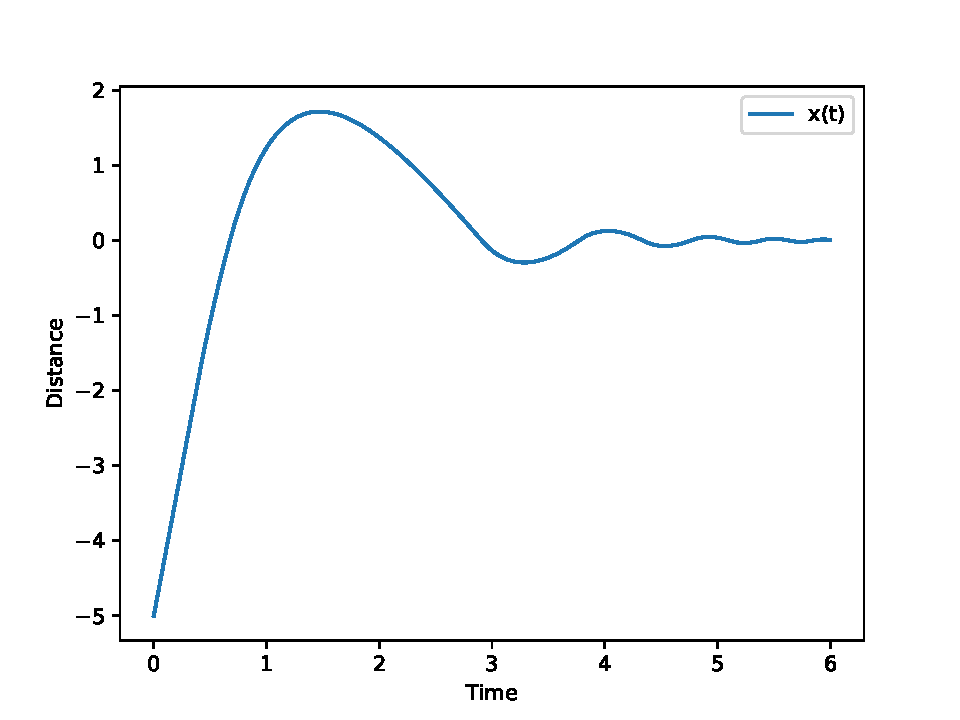
\includegraphics[scale=.7]{plot_integrated_v0_8.pdf}
    \caption{Plot of $x(t)$ for $t\in[0, 6]$}
    \label{fig:fig_i}
\end{figure}

We observe that the atom moves into the trap and continues past $x=0$. It will then experience a force in negative $x$-direction, which accelerates it towards $x=0$ again. Since $F_0$ is not conservative, the motion observed follows damped harmonic motion. It ends in $x=0$ as this is the only stable equilibrium point. 

\newpage
\section{}
Now, we simulate with $v_0 = 10.0$ and $x=-5$.
\begin{figure}[h!]
    \centering
    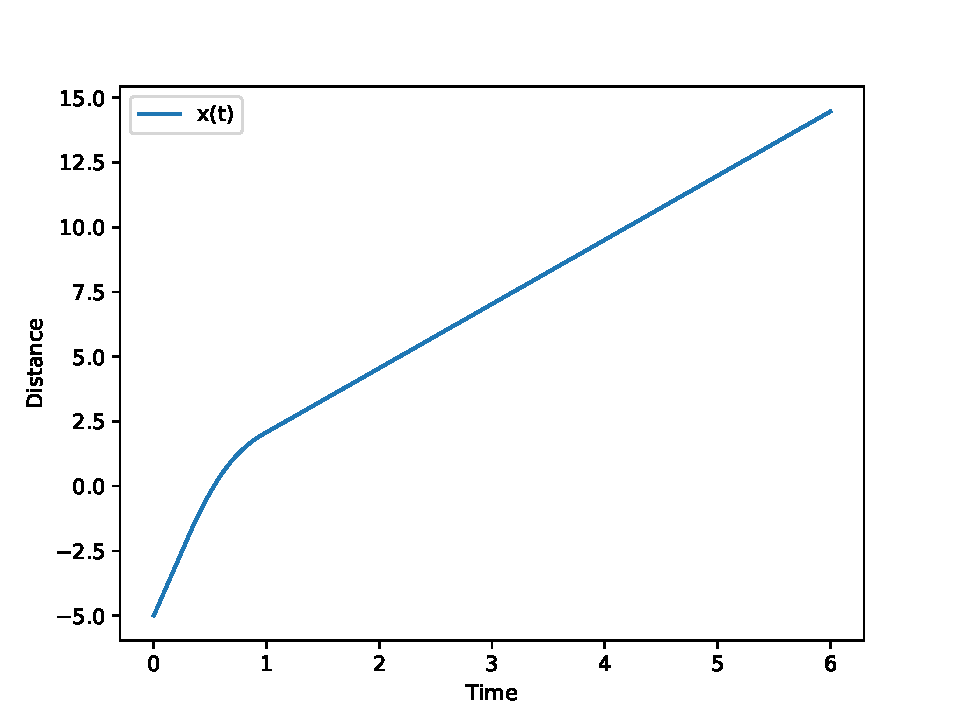
\includegraphics[scale=.7]{plot_integrated_v0_10.pdf}
    \caption{Plot of $x(t)$ for $t\in[0, 6]$}
    \label{fig:fig_j}
\end{figure}

In this simulation, the atom has enough energy to escape the trap on the other side. When it reaches $x=x_0=2$ the force on the atom will be 0, and it will continue forever with constant velocity. 

\end{document}
